\chapter{Results of Workflow Validation}\label{chap:results}
The Galaxy workflows are validated using real-world datasets from different laboratories. The analysis results for each workflow with complying test samples are described below.

\section{Poxvirus Workflow with Lumpy Skin Disease Virus Datasets}
We employed our pipeline using a tiling amplicon approach with masked reference sequences for each half genome to ensure an unambiguous mapping to the identical two \ac{ITR} regions of the poxvirus genome. Two public \ac{LSDV} samples, 20L70 (MZ577075.1) and 20L81 (MZ577076.1), that were sequenced using a primer scheme with two primer pools are used and retrieved from GenBank on 10\textsuperscript{th} April, 2023. Collected from cattle in 2020 during a lumpy skin disease outbreak in Northern Vietnam (20L70\_Dinh-To/VNM/20 and 20L81\_Bang-Thanh/VNM/20), both samples were sequenced on a MiSeq System using a Nextera XT library preparation kit. \\
The used \acs{CaPV} primer scheme in \ac{BED} format contains information about the primer pairs used for the amplicons. Each primer pair has one positive and one negative strand primer, indicated by the strand in the sixth column and by the \textit{LEFT} and \textit{RIGHT} label in the name. Primers are labeled in an alternating way: \textit{pool1} primer pairs are denoted as \textit{pool1a} and \textit{pool1b}. We use the same method for \textit{pool2} with \textit{pool2a} and \textit{pool2b}. We reuse the \textit{SCORE} column from the \ac{BED} file to unambiguously identify primer and strand for each amplicon. The annotated primer scheme for \ac{CaPV} is part of the workflow run to which links are provided in Supplementary~\secref{sec:apx-aiv-links}. The \ac{LSDV} ``Neethling'' strain was used as reference genome (NC\_003027.1, retrieved on GenBank 10\textsuperscript{th} April, 2023) for mapping. The raw FASTQ files for each sample were quality trimmed with \texttt{fastp} and mapped to each half-masked reference, which is explained in detail below. Preprocessing with default \texttt{fastp} settings includes automatically detected adapter trimming, a quality filter to discard reads below an average quality of Q15, with more than 5 uncalled (N) bases and 40\% unqualified bases, a length filter to discard reads below a threshold of 30, automatic trimming of polyG tails for Illumina NextSeq/NovaSeq data and a minimum length of 10 to detect polyG tails.
\\

\setlength{\tabcolsep}{16pt}
\renewcommand{\arraystretch}{1.3}
\begin{table}[ht!]
    \centering
    \begin{tabular}{lcc}
    \toprule
    \textbf{Output Metric}                      & \textbf{20L70}     & \textbf{20L81}     \\ \midrule
    Paired-end raw reads                        & 863 820            & 1 016 168          \\ 
    Paired-end reads after quality trimming     & 856 138            & 947 064            \\ \midrule
    Proportion of reads mapping to reference    & 99.6\%             & 77.3\%             \\ 
    Proportion of reference covered             & 99.68\%            & 99.68\%            \\ \midrule
    Mean coverage                               & 2 705.2\texttimes & 2 411.4\texttimes \\ 
    Alignment error rate                        & 1.25\%             & 1.30\%             \\ \bottomrule
    \end{tabular}
    \caption{Metrics after preprocessing and mapping for datasets 20L70 and 20L81.}
    \label{tab:4-pox-metrics}
\end{table}

\begin{figure}[ht!]
    \centering
    \hspace*{-8pt}
    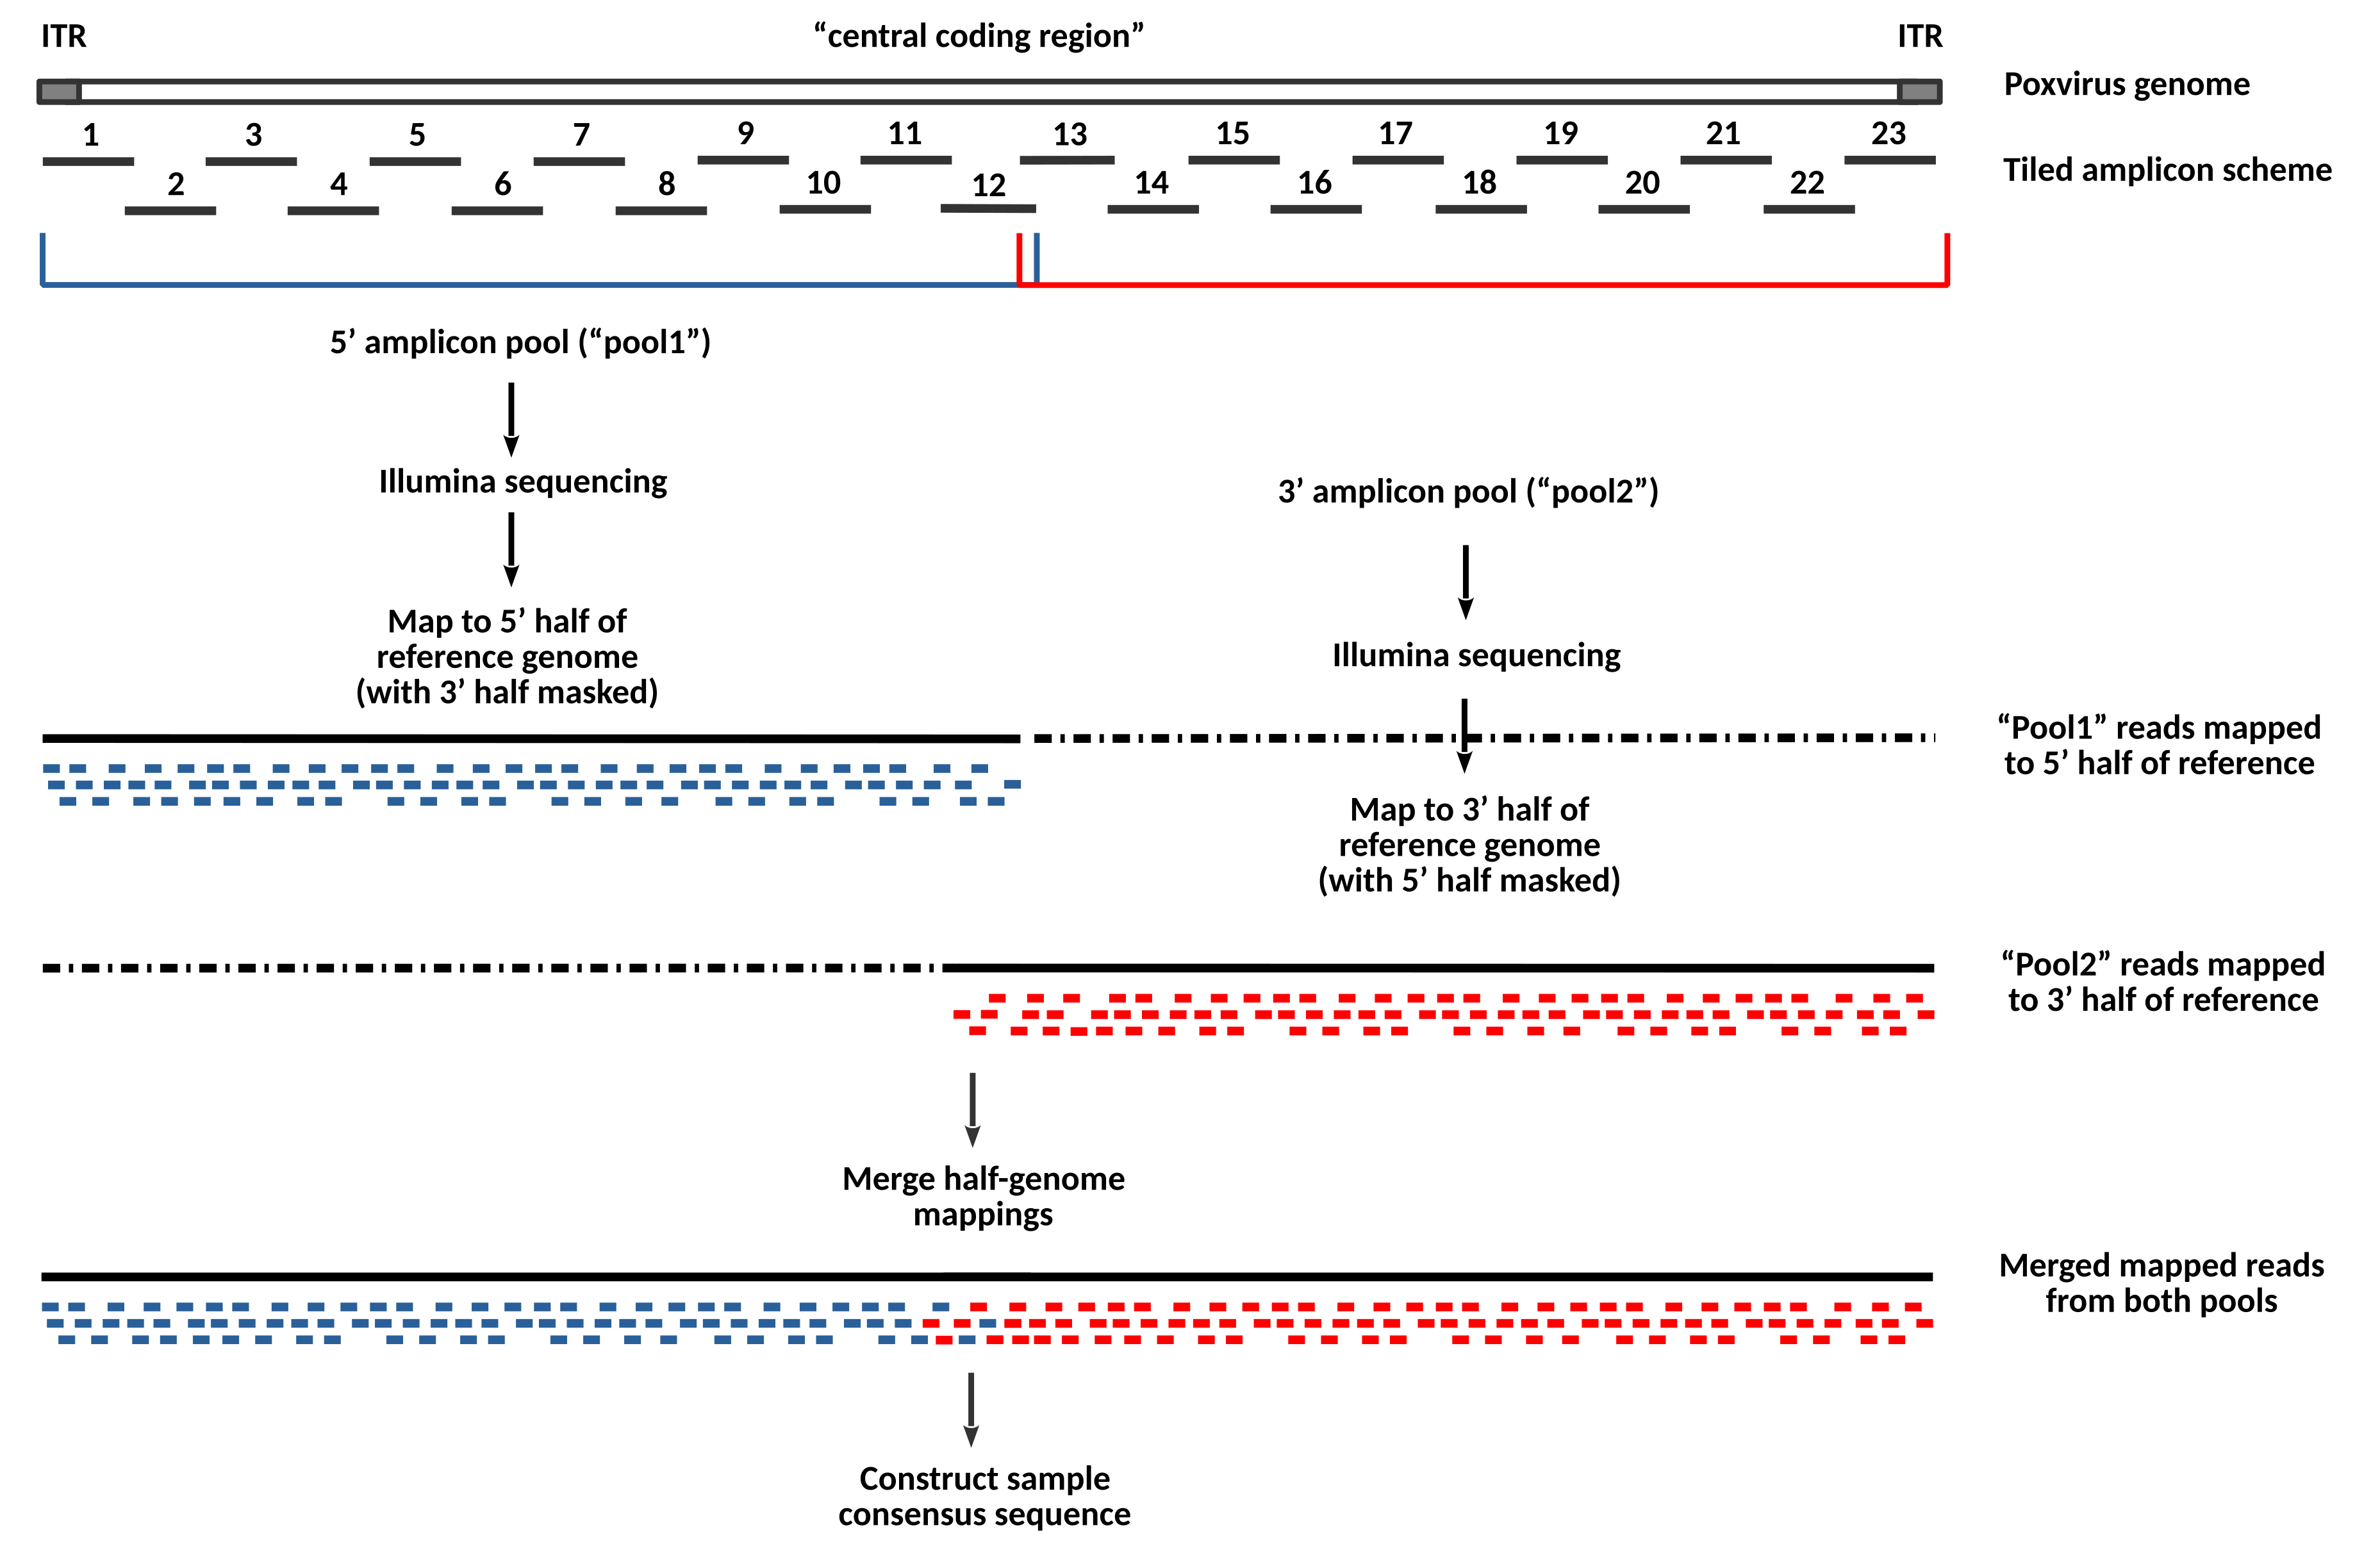
\includegraphics[width=1.1\textwidth]{media/4-pox-ampl-fig.png}
    \caption[Tiling amplicon scheme used in poxvirus workflow.]{Tiling amplicon scheme emphasising masking of the reference, mapping in two pools and merging of mappings with almost no overlap. Source: adapted from \todo{Poxvirus tutorial}}
    \label{fig:4-pox-ampl}
\end{figure}
The used primer scheme contains a total of 23 primers, while the first set of 12 primers covers the 5' genome end labeled with \textit{pool1}, and the remaining 11 primers cover the 3' genome end, labeled with \textit{pool2} as depicted at the top in blue (\textit{pool1}) and red (\textit{pool2}) in~\figref{fig:4-pox-ampl}. This scheme was designed for the tiling amplicon approach all three members of Capripoxviruses, which includes the \ac{LSDV} sample. To use the primer scheme with \ac{SPPV} or \ac{GTPV} samples, the primer positions need to be shifted to the correct coordinates.\\
The used primer scheme is provided in the Galaxy history of the test runs and is available via links in Supplementary~\secref{sec:apx-pox-links}. Inspection of the masking intervals for N-masking the reference confirms that the right-most position of Ns of masking the 5' half (i.e. preparing the reference for mapping \textit{pool2} reads) is the minimal start position of \textit{pool2} primers (``1 -- 79081'', and 79081 being the start position of primer 13). Accordingly for N-masking the reference for mapping of \textit{pool1} reads, the position of the right-most primer end of \textit{pool1} primers (primer 12) is 80202, resulting in the interval ``80202 -- 150773''. This is clearly visible in~\figref{fig:4-lsdv-read-groups}, where reads from \textit{pool1} are labeled in red and \textit{pool2} in blue, and mapped to the same reference sequence with different masked parts. As expected, the coverage in the region where reads from both pools mapped to is higher.\\
The final position is the maximal end position and the total length of the reference sequence. Since the reference genome and primer scheme are the same for both datasets 20L70 and 20L81, the N-masked references are used for both mappings. Mapping of each pool is done with \texttt{BWA-MEM} and default settings for Illumina-sequenced reads, using the N-masked reference for \textit{pool1} and \textit{pool2} respectively. This results in a mapping with a small overlap in the central part of the genome, where primer 12 ends and primer 13 starts as indicated in the top of~\figref{fig:4-pox-ampl}. After merging the mappings with \texttt{Samtools merge}, statistics for preprocessing and mapping are reported and summarised in~\tabref{tab:4-pox-metrics}. \figref{fig:4-lsdv-read-groups} shows a screenshot from \ac{IGV}, where the mapping of reads from \textit{pool1} (red) and \textit{pool2} (blue) are merged and demonstrate a higher coverage in the overlapping part of the reference sequence which was mapped to in both pools. For both samples 20L70 and 20L81, almost the complete reference genome was covered during mapping (99.68\%) with a mean coverage of {2705.2\texttimes } and {2411.4\texttimes } respectively. Primer end positions of \textit{pool2} primers are highlighted with blue circles and mark the start position of the overlapping region and the end of the masking of the reference sequence for \textit{pool2}.
\\

\begin{figure}[ht!]
    \centering
    \hspace*{-24pt}
    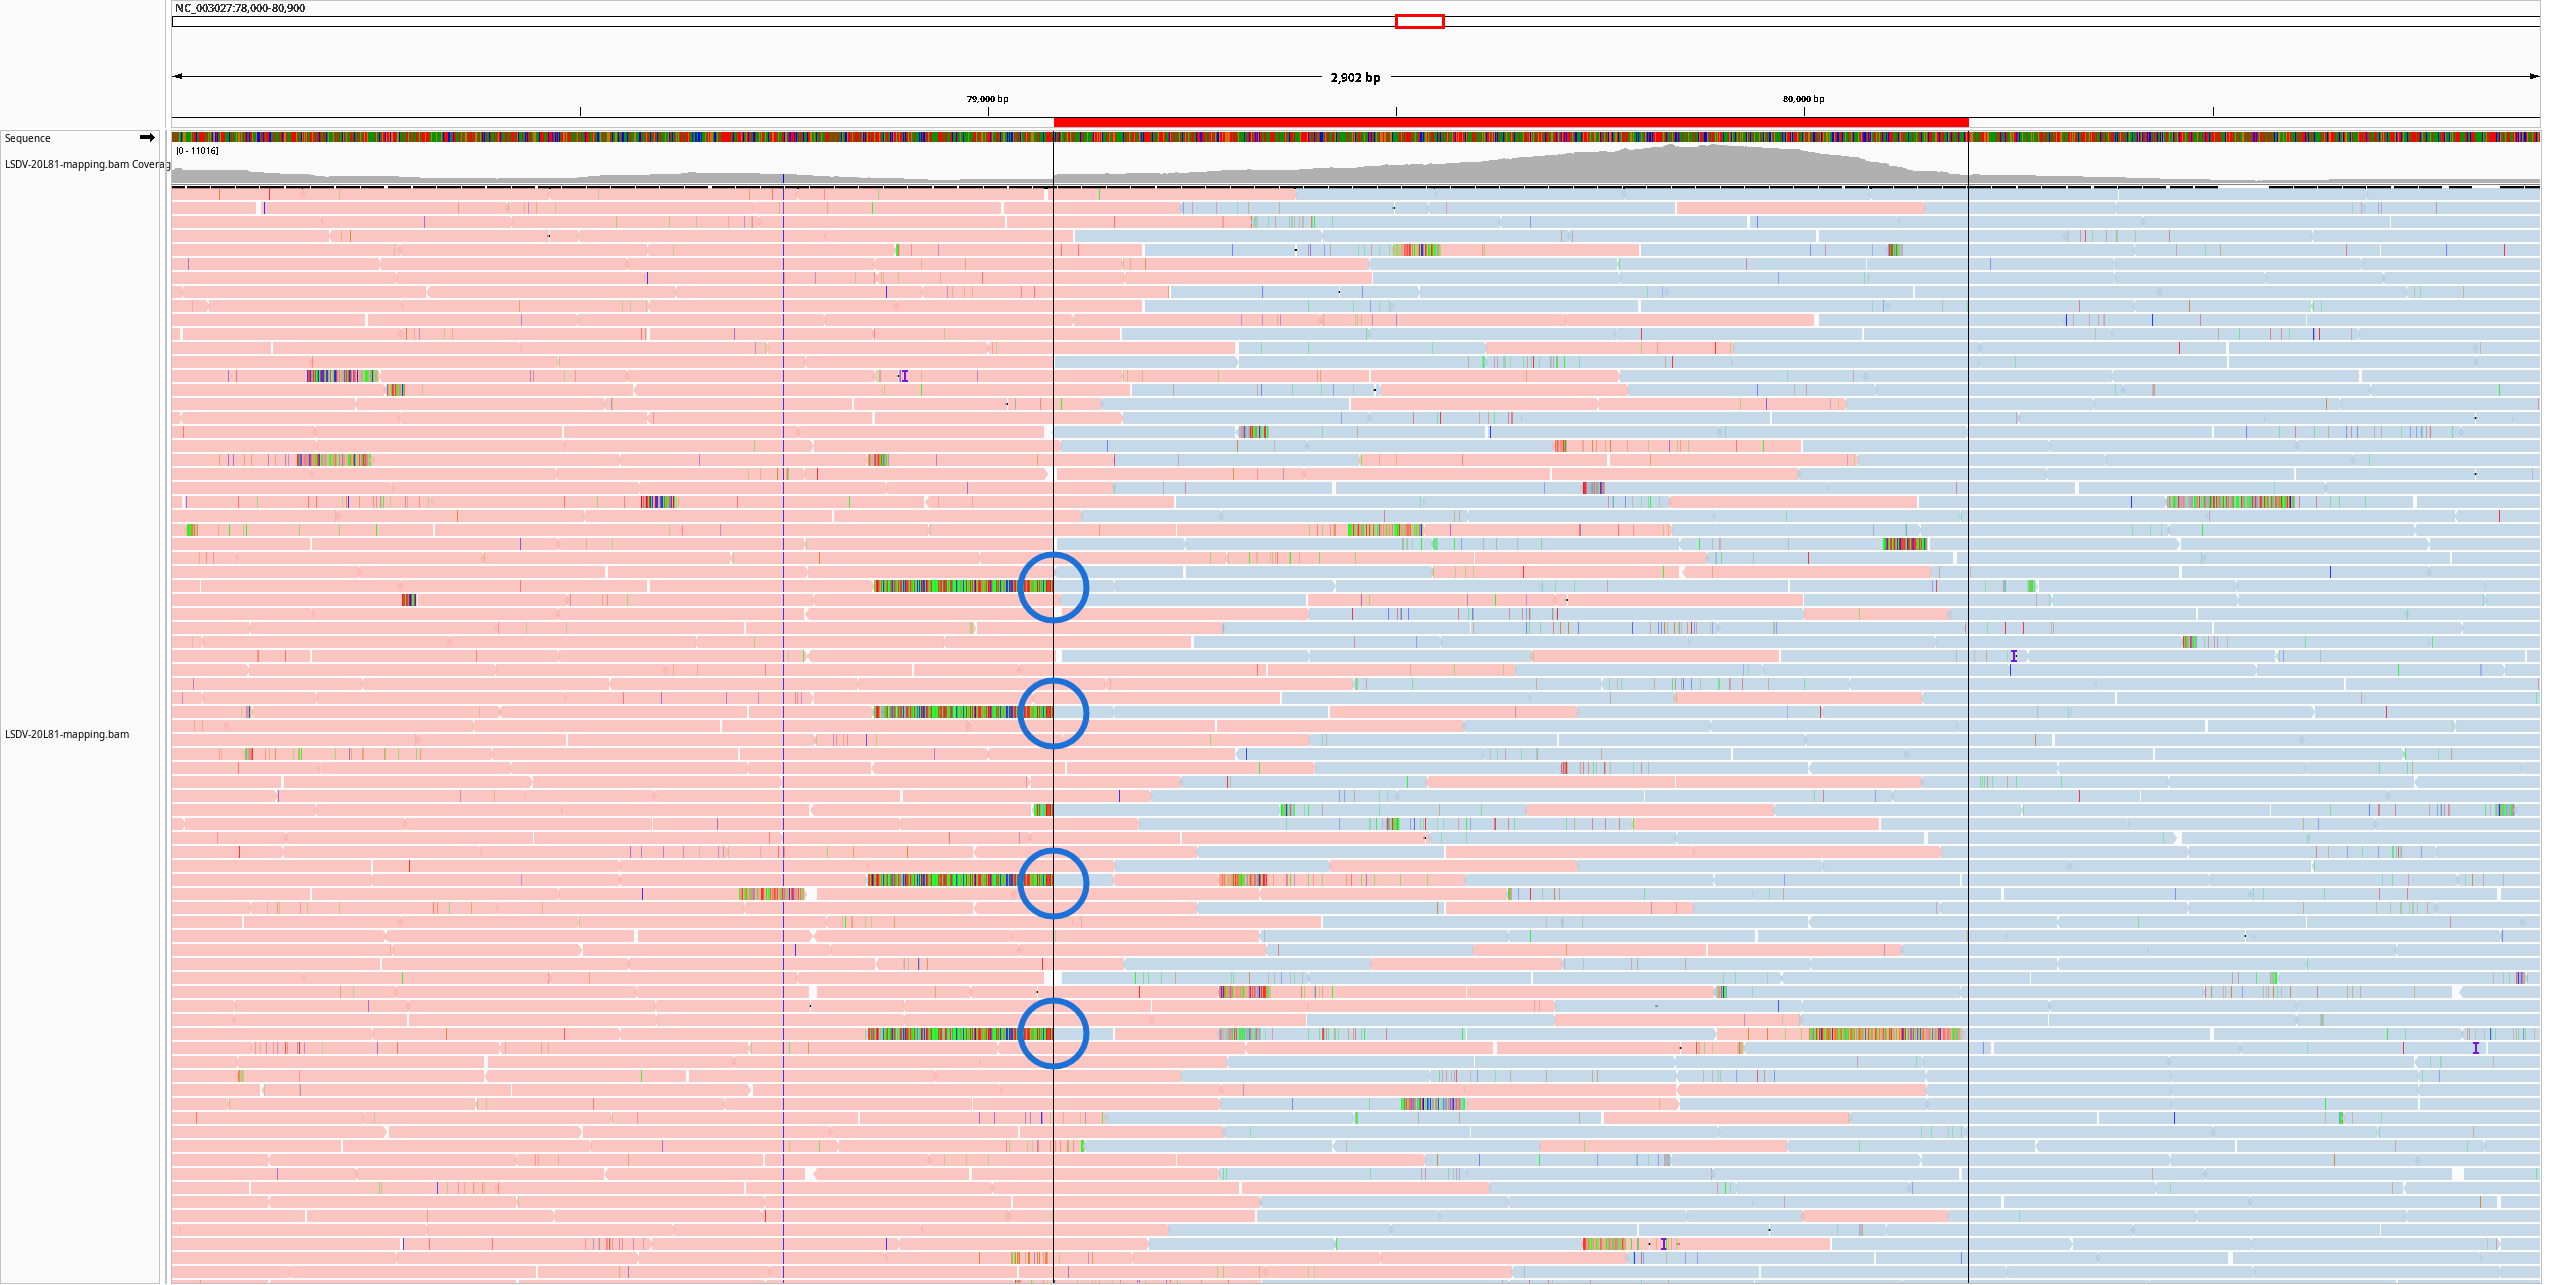
\includegraphics[width=1.1\textwidth]{media/4-lsdv-alig-20L81-c.png}
    \caption[Overlapping reads region of LSDV mapping in 20L81 sample.]{Overlapping, seamlessly merged mapping region of the two amplicon pools of the 20L81 sample. Coloured reads indicate read groups from \textit{pool1} (red) and \textit{pool2} (blue), primers are soft-clipped and end where the mapping of \textit{pool2} reads starts, as marked with blue circles for primer 13 to which four reads from \textit{pool2} bind. More primers may bind outside of the cropped snapshot.}
    \label{fig:4-lsdv-read-groups}
\end{figure}

The merged mapping of both read pools was quality trimmed with \texttt{iVar trim} to remove primers and mapped reads with a length of less than 30 bp. The remaining reads were used for full-length consensus sequence construction with \textit{iVar consensus}, developed for amplicon-based sequencing data. Inspection of the consensus sequences for both samples shows that apart from low coverage regions in the 5' front and 3' tail due to ampliconic sequencing, a consensus sequence was produced and a base at each position could be found. A base could not be called in the consensus at the first 264 positions in both the 20L70 and 20L81 sample, which corresponds to the primer binding site on the forward strand, and no bases at the last 268 positions indicate the remaining part where the last primer on the reverse strand starts. This was expected due to ampliconic sequencing where the first primer ends at genomic position 264, and where the target sequence starts. The workflow ends by producing a collection of the per-sample consensus sequences.

\subsubsection*{Poxvirus Workflow Validation using other CaPV Reference Sequences}
Until 2017, genomic analysis of different \ac{LSDV} samples from all over the world suggested very limited genomic variation. The two phylogenetic clusters that were thought to be stable: the Neethling-based strain (used for vaccine development) and a wild-type strain~\cite{biswas2020extended}. In 2018, a report has been filed from a vaccine-like field isolate that revealed the presence of multiple recombination sites within the sample while one of the found parental strains was the Neethling vaccine strain (referred to as Saratov strain as in~\secref{sec:2-pox})~\cite{sprygin2018analysis}. Following current sequencing efforts, the existence of more recombinant clusters has been demonstrated from field isolates that took the Neethling-based vaccine. Analysis of this vaccine revealed the presence of multiple Capripoxviruses within the sample: the Neethling-vaccine strain, a KSGP-based vaccine strain, a \ac{GTPV} strain from Sudan and most importantly other different recombinants between KSGP and Neethling strains. These studies suggest that this recombinant \ac{LSDV} strain that currently spreads in Asia is likely caused by a vaccine spillover~\cite{vandenbussche2022recombinant}. The Kenyan Sheep and Goat Pox (KSGP) strain was first detected in \ac{LSDV}-infected sheep and goats from Kenya, although it has been used for sheeppox and goatpox vaccines~\cite{tuppurainen2014characterization}. \\
The test samples 20L70 and 20L81 are shown to be from this recombinant vaccine strain, and in order to validate the presence of recombinant sites within these samples, we compare the recombinant sites that differentiate the strains from each other. For this purpose, we run the poxvirus workflow with the two \ac{LSDV} samples, but use reference sequences from other clades of the Capripoxviruses and thereby highlight the recombinant sites relative to the recombinant Neethling-vaccine strain.

\setlength{\tabcolsep}{8pt}
\renewcommand{\arraystretch}{1.3}
\hspace*{-24pt}
\begin{table}[ht!]
    \centering
    \begin{tabular}{@{}lccccc@{}}
    \toprule
                            & \multicolumn{1}{l}{\textbf{\begin{tabular}[c]{@{}l@{}}LSDV-\\ Neethling\end{tabular}}} & \multicolumn{1}{l}{\textbf{\begin{tabular}[c]{@{}l@{}}LSDV-\\ KSGP\end{tabular}}} & \multicolumn{1}{l}{\textbf{\begin{tabular}[c]{@{}l@{}}LSDV-\\ Herbivac\end{tabular}}} & \multicolumn{1}{l}{\textbf{SPPV}} & \multicolumn{1}{l}{\textbf{GTPV}} \\ \midrule
    \textbf{\begin{tabular}[c]{@{}l@{}}LSDV-Neethling\\\textnormal{(NC\_003027.1)}\end{tabular}} & 0                                                                                      & 0.0006                                                                            & 1.1                                                                                   & 2.1                               & 1.8                               \\
    \textbf{\begin{tabular}[c]{@{}l@{}}LSDV-KSGP\\\textnormal{(KX683219.1)}\end{tabular}}      &                                                                                        & 0                                                                                 & 1.1                                                                                   & 2.1                               & 1.8                               \\
    \textbf{\begin{tabular}[c]{@{}l@{}}LSDV-Herbivac\\\textnormal{(KX764644.1)}\end{tabular}}  &                                                                                        &                                                                                   & 0                                                                                     & 2.1                               & 1.9                               \\
    \textbf{\begin{tabular}[c]{@{}l@{}}SPPV\\\textnormal{(NC\_004002.1)}\end{tabular}}           &                                                                                        &                                                                                   &                                                                                       & 0                                 & 2.4                               \\
    \textbf{\begin{tabular}[c]{@{}l@{}}GTPV\\\textnormal{(NC\_004003.1)}\end{tabular}}           &                                                                                        &                                                                                   &                                                                                       &                                   & 0                                 \\ \bottomrule
    \end{tabular}
    \caption[Maximum Likelihood Distance matrix of CaPV strains.]{Distance Matrix based on a maximum likelihood criterion of all clades within the CaPV genus. The LSDV clades are more closely related with each other than SPPV and GTPV, while the LSDV Neethling and KSGP strains are almost identical, and the recombinant LSDV-Herbivac vaccine strain is distinct.}
\label{tab:4-capv}
\end{table}

To determine the relationship among the used reference sequences, a distance matrix as shown in~\tabref{tab:4-capv} shows the four different known clades within the Capripoxvirus genus. While the \ac{LSDV}-Neethling strain and KSGP strain are very closely related, the recombinant \ac{LSDV}-vaccine strain differs from this clade. \ac{SPPV} and \ac{GTPV} clades are shown to be more different to the \ac{LSDV} clades. By converting a multiple sequence alignment of the reference used for mapping, the constructed consensus sequences and the \ac{LSDV}-vaccine reference (Herbivac, GenBank: KX764644.1) to a \ac{VCF} file and detect variants relative to the vaccine strain. The tool \texttt{faToVcf} was wrapped as part of this work to make it accessible from within Galaxy. The tool was initially published by the University of California, Santa Cruz (UCSC) and generates a \ac{VCF} file.\\
Using this approach to compare the consensus sequences, constructed by mapping the 20L70 and 20L81 sample reads to other \ac{CaPV} reference sequences, and comparing variation sites relative to the \ac{LSDV}-vaccine strain, the found sites show different locations that differentiate the clade from the recombinant strain. The used primer scheme was adapted for  mapping to \ac{SPPV} and \ac{GTPV} due to shorter genome lengths and different primer locations.Although the \texttt{faToVcf} tool is not capable of displaying indels, it clearly shows unmapped regions and the \acp{SNP} relative to the vaccine strain.

SPPV compared to recomb. LSDV vaccine strain (Ns): (20L81)
- 18,479-18,498
- 110,083-110,106

SPPV compared to recomb. LSDV vaccine strain (Ns): (20L70)
- 18,477-18,505
- 110,090-110,113
- 129,582-129,583 (low cov.?)

The impact of the found \acp{SNP} was not examined because a gene annotation file for poxviruses with genomic features on th amino acid layer was not available.


\section{AIV Workflow with H4N6 and H5N8 Samples}\label{sec:4-aiv}
\setlength{\tabcolsep}{14pt}
\renewcommand{\arraystretch}{1.3}
\begin{table}[ht!]
    \centering
    \begin{tabular}{lcc} 
    \toprule
    \textbf{Output Metric}                                                                & \textbf{H4N6} & \textbf{H5N8} \\ \midrule
    Paired-end raw reads                                                                  & 1 537 722                  & 858 610                    \\ 
    \begin{tabular}[c]{@{}l@{}}Paired-end reads after quality\\trimming\end{tabular}      & 1 507 396                  & 830 176                    \\ \bottomrule
    \end{tabular}
    \caption[Metrics after preprocessing of H4N6 and H5N8 samples.]{Metrics about Illumina reads before and after preprocessing of H4N6 and H5N8 samples.}
    \label{tab:4-aiv-metrics}
\end{table}

The \ac{AIV} Illumina workflow on the Galaxy platform was evaluated using two field isolates provided by Sciensano, the Belgian national health institute. The isolates were extracted in Belgium in 2020 from an H4N6 infected magpie (EPI\_ISL\_7593059) and an H5N8 infected duck (EPI\_ISL\_7596571). For reasons of readability, we refer to the samples as H4N6 and H5N8 samples. The two samples were sequenced on an Illumina platform in paired-end mode and are utilised one sample per workflow run on Galaxy. For the \ac{AIV} Illumina workflow, a reference database in FASTA format is required as a collection, i.e. a list of one dataset per \ac{AIV} segment, which is uploaded in Galaxy. The used database contains multiple sequences per segment as described in~\secref{sec:3-aiv-ref}. The amount of sequences and distribution of subtypes within each segments suggests that variation within each subtype is generally captured well with the given database. Due to the filtering criteria, not all eight segments of one sample were found suitable for the database.\\
After starting the workflow, the paired-end reads were preprocessed and serve as query reads for \texttt{VAPOR}. Metrics of before and after preprocessing are shown in~\tabref{tab:4-aiv-metrics} and count more than 1.50 million reads after preprocessing for the H4N6 sample and 0.83 million reads for the H5N8 dataset. Since the reference database contains eight FASTA files in a collection, \texttt{VAPOR} runs once per dataset and outputs the highest scoring sequences per segment, which represents the most similar sequences from the database compared to the query sequences. \\

\setlength{\tabcolsep}{8pt}
\renewcommand{\arraystretch}{1.3}
\begin{table}[ht!]
    \centering
    \hspace*{-16pt}
    \begin{tabular}{@{}lcccc@{}}
    \toprule
    \multicolumn{1}{l}{\textbf{Segment}} & \multicolumn{2}{c}{\textbf{Proportion of query bases in reads}}                             & \multicolumn{2}{c}{\textbf{AIV subtype of hit}}                                         \\ \midrule
                                         & \multicolumn{1}{l}{\textbf{H4N6 sample}} & \multicolumn{1}{l}{\textbf{H5N8 sample}} & \multicolumn{1}{l}{\textbf{H4N6 sample}} & \multicolumn{1}{l}{\textbf{H5N8 sample}} \\ \cmidrule(l){2-5} 
    HA                                   & 98.7\%                                    & 100.\%0                                      & H4                                       & H5                                       \\
    NA                                   & 98.7\%                                    & 100.0\%                                      & N6                                       & N8                                       \\ \bottomrule
    \end{tabular}
    \caption[Results of VAPOR run with AIV test samples.]{The best scoring sequence of the VAPOR run for each AIV test samples, indicating a perfect match (100\% of the query bases are in the reads) of the HA and NA segments of the H5N8 sample sequence, and almost all query bases of the H4N6 sample in the found sample.}    
\label{tab:4-aiv-vapor}
\end{table}

The \texttt{VAPOR} search was able to successfully identify the avian influenza virus subtypes present in each sample: for the H5N8 sample, the most similar sequence of HA segment origins from a sample with the H5 subtype, while the most similar sequence of the NA segment origins from a sample with the N8 subtype. Both found gene sequences contain 100\% of the input reads. Similarly, the H4N6 sample was correctly identified with concordance of query bases of 98.7\% each. The results of the \texttt{VAPOR} run for the HA and NA genes are summarised in~\tabref{tab:4-aiv-vapor}. \\
Consensus sequences for each genome segment were constructed with \texttt{iVar consensus} and while a consensus could be found at each position, the produced consensus sequences are 100\% identical to the originally assembled reads that were uploaded to \ac{GISAID} by the Sciensano laboratory from the same sample (EPI\_ISL\_7593059 and EPI\_ISL\_7596571). Due to slightly different genome sizes of the reference sequence used for mapping compared to the assembly, the resulting consensus sequences in the \ac{AIV} workflow are shorter than the assembled sequences on \ac{GISAID}. The consensus sequence for the \ac{HA} segment of the H4N6 sample is differing in 1 bp in the 5' end, and 4 bp in the 3' end. The consensus sequence constructed for the \ac{NA} gene misses 18 bp compared to the assembled sequence on \ac{GISAID} in the 5' end and 33 bp in the 3' end. Similarily, the \ac{HA} consensus sequence of sample H5N8 is 28 bp shorter in the front and 44 bp shorter in the end. The \ac{NA} consensus sequence differs in 20 and 28 bp in the front and tail. These differences indicate the missing \acp{UTR} on the whole-length genome. While the hybrid reference that was compiled from the eight influenza segments contains complete segments including start and stop codons, which is a criterion for each sequence to be part of the reference database, the aligned consensus sequence does not contain the \acp{UTR} at the 5' and 3' ends as opposed to the \textit{de novo} assembled sequences uploaded to \ac{GISAID}. This was validated by running the \texttt{getorf} tool in Galaxy and reporting the \acp{ORF} as nucleotide sequences between start and stop codons. This analysis showed the presence of full \acp{ORF} in each segment in both test samples.
\\
Other workflow outputs for the \ac{AIV} samples include plots that visually emphasise \acp{SNP} relative to the top hits of the \texttt{VAPOR} run, indicating the most similar sequences from the reference collection. The plots for the \ac{HA} and \ac{NA} genes for the H4N6 sample (\figref{fig:apx-aiv-snipit-s4}) show 30 \acp{SNP} compared to the first sequence which was also used as reference for mapping (LC121412.1) and 31 \acp{SNP} compared to the second best result (MK192399.1). Similarly, the \ac{NA} gene consensus sequence has 29 \acp{SNP} compared to the reference sequence (MW19994.1). For the H5N8 sample, the \texttt{VAPOR} run found a sequence with 100\% of the query bases in the reads, and therefore the number of \acp{SNP} is expected to be low. Supplementary~\figref{fig:apx-aiv-snipit-s8} shows there is one \ac{SNP} in the \ac{HA} gene compared to the reference (MZ166252.1) at position 1002 and one \ac{SNP} at position 497 compared to the \ac{NA} reference sequence (MZ166270.1). The \acp{SNP} indicate point mutations or mapping errors, low coverage or close calls during consensus sequence construction. \\
A protein FASTA file containing gene annotations is generated based on the consensus sequence with \texttt{Prokka} and can be used for detailed gene expression analysis. Changes on the amino acid level give valuable insights into the adaptation of the virus and to compare differences among strains in more detail. In virology, working on amino acid level is more common than with nucleotides alone. The protein FASTA file can be downloaded or used within Galaxy.\\
Phylogenetic classification relative to the 30 most similar sequences in the \ac{AIV} reference database, queried by \texttt{VAPOR}, is done for each segment to reveal temporal and geographical relations of the isolate. Generated phylogenetic trees with \texttt{IQ-Tree} are depicted in Supplementary Figures~\ref{fig:apx-aiv-trees-s4} and~\ref{fig:apx-aiv-trees-s8}. The trees are unrooted and for the \ac{HA} gene of the H4N6 sample, shows the nearest clade being from an isolate which is a H4N6 infected mallard from the Netherlands, taken in 2017, and for the \ac{NA} a single and very early split is made where the gene is clustered to a H6N6 infected duck from Hunan, China. The obtained results for the H5N8 sample show clustering of both the \ac{HA} and \ac{NA} genes with sequences from a H5N8 infected mule duck from France, taken in 2020 and 2021.\\
Users of the workflow with real-world samples could investigate in more detail by uploading their own reference collection and hereby finding links to other sequenced samples from previous outbreaks in their region. The depth of the split in a phylogenetic tree can indicate the degree of relatedness between the sample and the other samples within that split. A deeper split suggests a closer relationship between the sample and the other samples in that particular branch.

\section{FMDV Workflows with Asia-1, A, SAT-1 and SAT-2 Samples}
The samples used for workflow validation are downloaded from the \ac{NCBI} and were chosen exemplatory for four of the seven different \ac{FMDV} serotypes. All four samples were sequenced on an Illumina NextSeq 550 platform. Two samples (Asia-1 serotype, SRR17960053 and A serotype, SRR18751245) were taken from infected cattle and buffalo during an outbreak in Pakistan from 2008 to 2012. One sample (SAT-1 serotype, SRR18685689) was isolated from buffaloes in Kenya in 2016 and plaque purified before sequencing, and the fourth sample (SAT-2 serotype, SRR9328470) was taken from an \ac{FMD} outbreak in Nigeria in 2014. \\
The results of before and after preprocessing of the raw reads are described in~\tabref{tab:4-fmdv-metrics}. The SAT-2 sample contains a very low number of reads with only 11 576 reads after preprocessing, however to show the ability of the developed workflows, it was kept in the test sample collection. 
\\

\setlength{\tabcolsep}{12pt}
\renewcommand{\arraystretch}{1.3}
\begin{table}[ht!]
    \centering
    \begin{tabular}{lcccc} 
    \toprule
    \textbf{Output Metric}                                                              & \textbf{Asia-1} & \textbf{A}                                           & \textbf{SAT-1} & \textbf{SAT-2}\\ \midrule
    Paired-end raw reads                                                                & 577 360         & 2 297 706                                            & 903 052        & 11 816        \\ 
    \begin{tabular}[c]{@{}l@{}}Paired-end reads after quality\\trimming\end{tabular}    & 561 280         & 2 112 856                                            & 806 712        & 11 576        \\ \midrule
    \begin{tabular}[c]{@{}l@{}}Length of assembled contigs\\with > 4000 bp\end{tabular} & 7 760            & \begin{tabular}[c]{@{}c@{}}12 133\\7 558\end{tabular}  & 7 329           & 7 696          \\ \bottomrule
    \end{tabular}
    \caption{Metrics about Illumina reads after preprocessing and \textit{de novo} assembly of Asia-1, A, SAT-1 and SAT-2 serotype reads.}
    \label{tab:4-fmdv-metrics}
\end{table}

After \textit{de novo} assembly with \texttt{rnaviralSPAdes}, contigs less than half the length of the \ac{FMDV} genome size were discarded. This resulted in one contig per sample for the \ac{BLAST}n search, except for the A serotype reads, for which two contigs were assembled. As the longer contig with 12 133 bases is far larger than the \ac{FMDV} genome size, a contamination or co-infection with another virus is indicated. The \ac{BLAST}n search was performed against the \ac{NCBI} nucleotide database to identify the closest viral sequence matches. The results of the \ac{BLAST}n search showed that all the contigs were closely related to \ac{FMDV} as listed in~\tabref{tab:4-fmdv-blast}. The highest sequence identity was observed for the Asia-1 serotype sample, with 96.74\% identity, followed by the A, SAT-1 and SAT-2 serotypes, with 94.87\%, 93.77\% and 91.42\% identity, respectively. These results were consistent with the clinical samples being positive for \ac{FMDV} infection and the specific serotype. However, the second long contig of the A sample resulted in a \ac{BLAST}n hit for pestivirus (formerly known as bovine viral diarrhea virus 1) with 93.162\% identity~\cite{smith2017proposed}. This suggests the presence of a co-infection with the pestivirus in the given sample. It shows that the presented workflow is capable of assembling and identifying other viruses present. For consensus sequence construction in the second \ac{FMDV} workflow, the assembled pestivirus contig is ignored and the reference sequence for mapping can be chosen from the \ac{FMDV} hits for the other contig in the \ac{BLAST}n search. This sample shows that during the workflow, the user is required to attentively check the results for plausibility and the reference selection process should not be automated without exact validation of the desired virus. Note that \ac{BLAST} runs on the Galaxy EU servers use a locally installed database to ensure replicability of experiments. Hence results on the web form of the \ac{NCBI} \ac{BLAST}n search may result in different hits due to a different and newer database state. In the megablast search made in this workflow, the \ac{NCBI} NT database from 22\textsuperscript{nd} January 2018 was used. The multisample run with the discussed samples of this first \ac{FMDV} workflow is provided in a Galaxy history and is available via link which is provided in Supplementary~\secref{sec:apx-fmdv-links}.

\setlength{\tabcolsep}{12pt}
\renewcommand{\arraystretch}{1.3}
\begin{table}[ht!]
    \centering
    \begin{tabular}{@{}lcccc@{}}
    \toprule
    \textbf{Sample} & \textbf{\begin{tabular}[c]{@{}c@{}}Alignment length\\{[}bases{]}\end{tabular} }   & \textbf{Query coverage} & \textbf{Identical matches} \\ \midrule
    A              & 7602   & 92.21\%  & 94.87\%      \\
    Asia-1         & 7690   & 99.10\%  & 96.74\%      \\
    SAT-1          & 7331   & 100.0\%  & 93.77\%      \\
    SAT-2          & 7669   & 99.65\%  & 91.42\%      \\ \bottomrule
    \end{tabular}
    \caption[Results of the BLASTn run with four FMDV samples.]{Results of the BLASTn run with four FMDV samples. Query coverage refers to the percentage of identical matches in the alignment compared to the BLASTn hit, hereby indicating the quality of the alignment. Alignment length describes the alignment compared to the query length, indicating how much of the query sequence is covered with the alignment.}
\label{tab:4-fmdv-blast}
\end{table}

In order to run the second workflow for reference-based mapping and consensus sequence construction for each of the four samples, the top \ac{BLAST}n hit of each sample is downloaded in FASTA format to be used as reference sequence for the respective sample. Except for the A sample, the top hit is a \ac{FMDV} genome sequence of the serotype of the query sample. In this case, user control is crucial for the selection of a representative reference sequence of the respective virus and not the contaminating viral sequence.\\
With the \texttt{NCBI Accession Download} tool, the sequence of each sample that has the highest similarity to the assembled contig is added to the Galaxy history and with \texttt{Collapse Collection} the FASTA file is extracted from the list to a single file, so that it is in the required format to start the second part of the \ac{FMDV} workflow.\\

\setlength{\tabcolsep}{8pt}
\renewcommand{\arraystretch}{1.3}
\begin{table}[ht!]
    \centering
    \begin{tabular}{@{}lllll@{}}
    \toprule
    \textbf{Output Metric}                                                            & \textbf{Asia-1}    & \textbf{A}          & \textbf{SAT-1}     & \textbf{SAT-2}   \\ \midrule
    \begin{tabular}[c]{@{}l@{}}Accession no. of\\reference\end{tabular}               & KM268898.1         & JN006722.1          & KM268899.1         & JX014256.1       \\ \midrule
    \begin{tabular}[c]{@{}l@{}}Proportion of reads\\mapping to reference\end{tabular} & 100\%              & 100\%               & 100\%              & 100\%            \\
    \begin{tabular}[c]{@{}l@{}}Proportion of reference\\covered\end{tabular}          & 99.67\%            & 100\%               & 98.16\%            & 99.60\%          \\ \midrule
    Mean coverage                                                                     & 1 525.9\texttimes & 15 895.5\texttimes & 9 302.8\texttimes & 188.0\texttimes \\
    Alignment error rate                                                              & 3.47\%             & 5.08\%              & 5.87\%             & 8.18\%           \\ \bottomrule
    \end{tabular}
    \caption{Quality and coverage metrics of the alignment in the second FMDV workflow.}
\label{tab:4-fmdv-map}
\end{table}

For each of the testing samples, the accession numbers used as reference sequence for mapping with \texttt{BWA-MEM} are listed in~\tabref{tab:4-fmdv-map} as well as quality and coverage measures after mapping. As expected due to the low number of reads, the SAT-2 sample had a low mean coverage of {188.0\texttimes } and a relatively high error rate of 8.18\% compared to the other samples. Consensus sequences are accurately obtained for the Asia-1 and SAT-1 sample that each contain low-coverage regions in the 5' and 3' ends, so the consensus was lost with decreasing coverage in both genomic ends. Sample A has its only low coverage region immediately adjacent to the polyA tail at positions 7626--7634. The Asia-1 and SAT-1 samples show additional low coverage regions adjacent to the polyC tract (Asia-1 sample: genomic positions 372--383; SAT-1: 321--335). Using the same coverage threshold for consensus calling for a sample with a low amount of reads like SAT-2, the coverage criteria were not met in several regions (genomic positions 1--37, 293, 346--528, 3605--3639 and 8039--9131). The consensus sequences can be found in the Galaxy histories of the respective workflow runs for each sample which are linked in Supplementary~\secref{sec:apx-fmdv-links}. \\
Part of the reported results after consensus construction is a summarising \acp{SNP} plot, produced by the \texttt{snipit} tool. Even though the emitted PNG is too large to display at once, it provides an overview of the distribution of \acs{SNP} relative to the reference sequence used for mapping. In case of a recombination event, where genetic material from two or more virus strains that are infecting the same cell combines to form a new strain, the distribution of \acp{SNP} in the plot would deviate from statistical expectations, in such that there occur regions of high genetic diversity or a sudden shift in allele frquency. Using the visual approach without further tools for identification or confirmation of recombination events is a fast method to detect recombination in the sample, however requires expertise in the expected pattern of variation based on the reference genome. Besides recombination events, the distribution of variation on the reference genome indicates how representative the reference sequence, selected based on the \ac{BLAST}n search, captures the aligned reads. If the reference sequence only covers a large part of the genome and not the entire length, it would be reflected in the plot by indicating large numbers of \acp{SNP}. In each \texttt{snipit} plot produced for the four test samples, a high number of \acp{SNP} are displayed, relating to the high mutation rate of \ac{FMDV}, yet not showing any irregularities that could indicate recombination events. The plots can be retrieved as part of the Galaxy histories of the test sample runs, which are linked in Supplementary~\secref{sec:apx-fmdv-links}.

\section{Workflow Profiling}
\todoit Assembly vs. mapping\\
for long/short genomes, for rnaviralSPAdes and BWA-MEM, compare CPU runtime and wall clock time, max.mem usage determines the scheduling on a cluster on galaxy (more requested memory means longer queuing times due to fewer available machines)

\begin{figure}[ht]
    \centering
	\begin{subfigure}[b]{1.1\textwidth}
        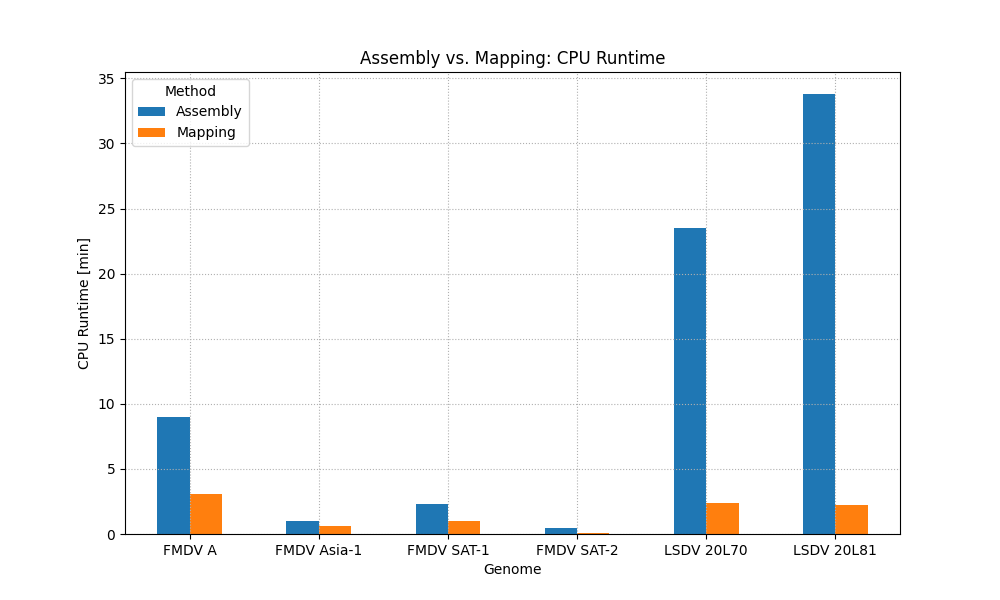
\includegraphics[width=1.0\textwidth]{media/4-profiling-cputime.png}
        \caption{Profiling of assembly versus mapping}
        \label{fig:4-profiling-cpu}
    \end{subfigure}
    \medskip
	\begin{subfigure}[b]{1.1\textwidth}
        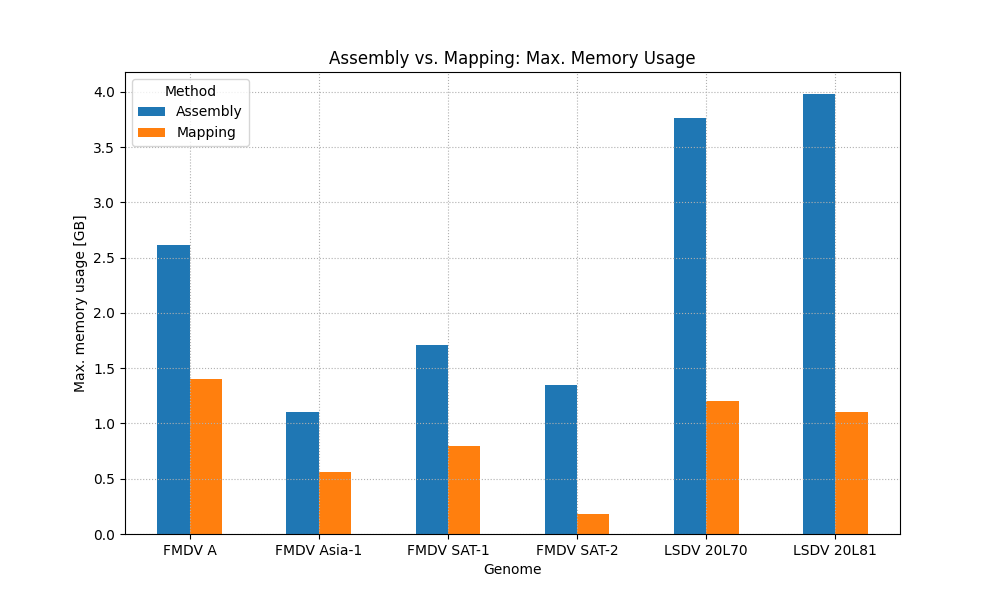
\includegraphics[width=1.0\textwidth]{media/4-profiling-maxmem.png}
        \caption{Profiling of assembly versus mapping}
        \label{fig:4-profiling-meem}
    \end{subfigure}
    \caption{Profiling}
\end{figure}
\begin{figure}[ht]\ContinuedFloat
    \centering
	\begin{subfigure}[b]{1.1\textwidth}
        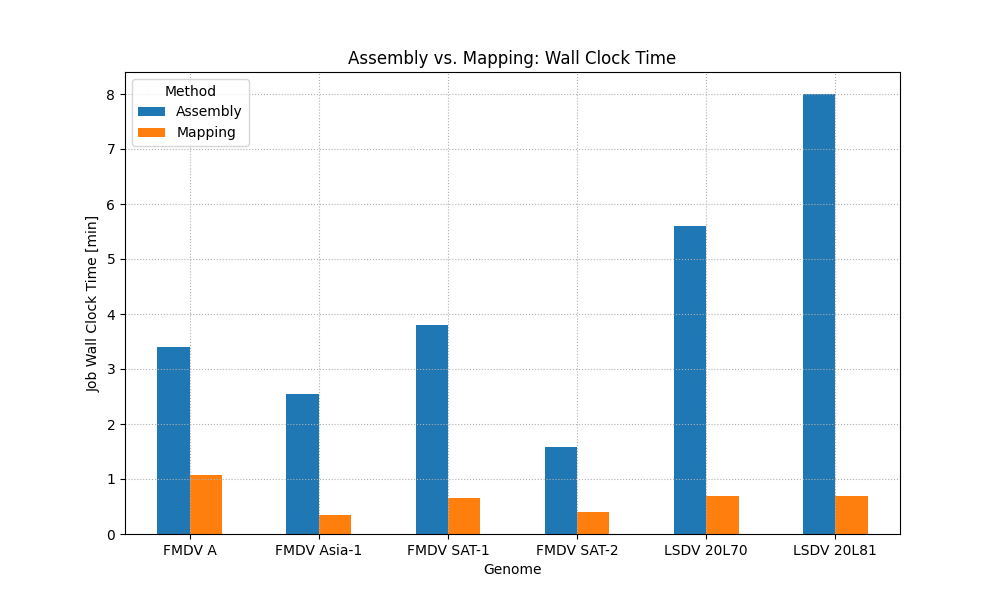
\includegraphics[width=1.0\textwidth]{media/4-profiling-wallclock.png}
        \caption{Profiling of assembly versus mapping }
        \label{fig:4-profiling-wallclock}
    \end{subfigure}
    \caption{Profiling (cont.)}
    \label{fig:4-profiling}
\end{figure}

on a locally installed galaxy server: depends on the cpu alone

% % smallest EC2 machine we could find is m5d.4xlarge (64 GB / 16 vCPUs / Intel Xeon Platinum 8175). 
% smallest EC2 machine we could find is m3.2xlarge (30 GB / 8 vCPUs / Intel Xeon E5-2670 v2 (Ivy Bridge/Sandy Bridge))

% poxv. wf less than 20min